\documentclass[c,8pt,xcolor...,x11names]{beamer}
\usepackage{icclslides}
\usepackage[latin1]{inputenc}
\usepackage[british]{babel}
\usepackage{amssymb}
\usepackage{latexsym}
\usepackage{rotate}
\usepackage{tikz}
\usepackage{verbatim}
\usepackage{colortbl}
\usepackage{booktabs}
\usepackage{ulem}
% \usepackage{arydshln}
%\usepackage{pdfpages}hord
\usepackage{graphicx} 
\usepackage{tikzsymbols}
\usepackage{tikz}
\usepackage{subcaption}
\usepackage[export]{adjustbox}
\usepackage{pdfpages}
\usetikzlibrary{positioning}

\tikzstyle{ele} = [circle, text centered, minimum width=1em, minimum height=3ex]

%% Uncomment to activate navigation symbols in the lower right of the pages:
\setbeamertemplate{navigation symbols}{}
%\setbeamercovered{transparent}

\renewcommand{\Myauthor}{Martin R\"obke}
\renewcommand{\Mytitle}{ Visualizing Dynamic Programming 
	On Tree Decompositions}
\usepackage{showexpl} 

\lstloadlanguages{[LaTeX]Tex} 
\lstset{% 
     basicstyle=\ttfamily\small, 
     commentstyle=\itshape\ttfamily\small, 
     showspaces=false, 
     showstringspaces=false, 
     breaklines=true, 
     breakautoindent=true, 
     captionpos=t 
} 

\begin{document}
\begin{frame}
	\customtitle
	\begin{list2}
		\item {\sc What} was the motivation
		\item {\sc What} could be used previously?
		\item {\sc Who} benefits from visualization?
		\item {\sc Challenges} and solutions
		\item {\sc What} could be developed next?
	\end{list2}
\end{frame}

%%%%%%%%%%%%%%%%%
\section{The task} % taken from Marek Seliger, Matthias Gerdts

\begin{frame}
	\frametitle{Task definition}

	Martin R\"obke
	
	Johannes Fichte
	
	Stefan Gumhold

\end{frame}

%%%%%%%%%%%%%%%%%%%%%%
\section{Motivation}

\begin{frame}
	\frametitle{Motivation}

\end{frame}

%%%%%%%%%%%%%%%%%%%%%%%
\section{Who should use this}
\begin{frame}
	\frametitle{Creating Visualization for:}
	\begin{minipage}{0.44\textwidth}
		\emph{Improving}
		\begin{itemize}
			\item examples for students
			\item debugging and improving interaction of complex data-structures
			\item hotspots
		\end{itemize}\medskip
		
	\end{minipage}
	\begin{minipage}{0.55\textwidth}
		\begin{figure}
			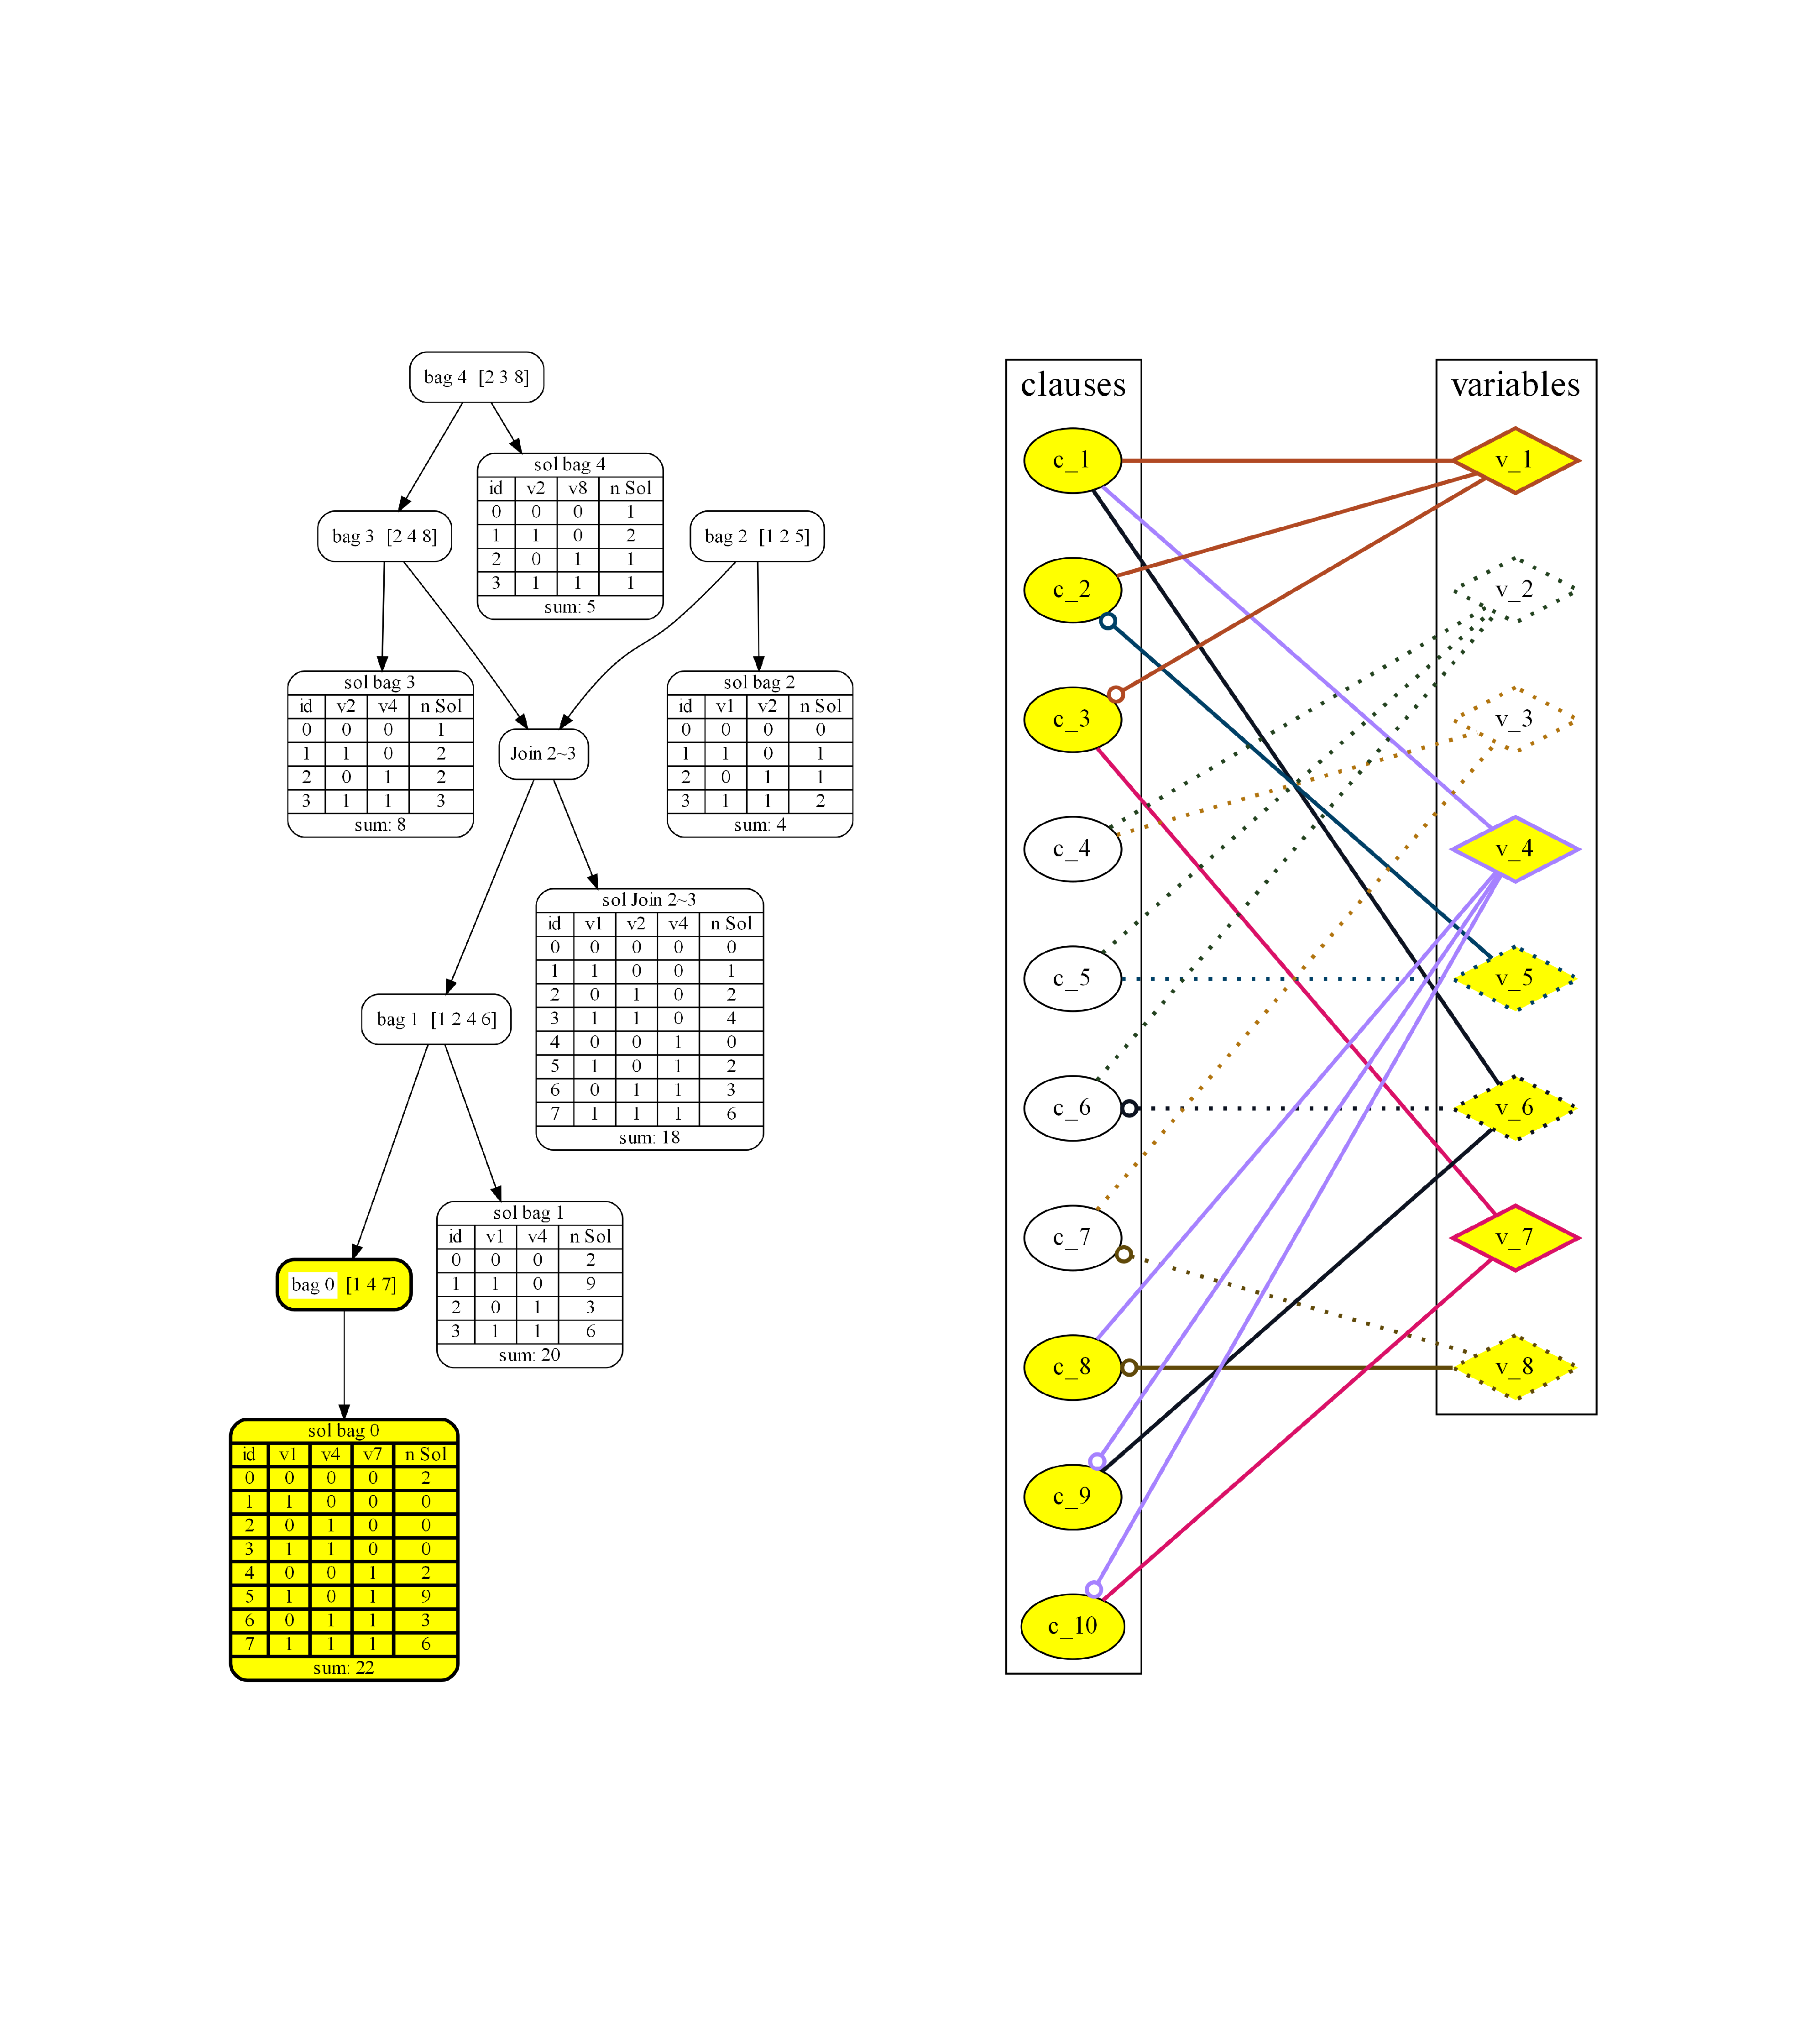
\includegraphics[width=\linewidth]{images/combined8.png}
		\end{figure}
	\end{minipage}
	
\end{frame}
%%%%%%%%%%%%%%%%%%%%%%%
\section{Other Visualization}
\subsection{Software}
\begin{frame}
	https://gephi.org/
%	Gephi is a tool for data analysts and scientists keen to explore and understand graphs. Like Photoshop? but for graph data, the user interacts with the representation, manipulate the structures, shapes and colors to reveal hidden patterns.

	https://tulip.labri.fr/TulipDrupal/
	
%	Written in C++ the framework enables the development of algorithms, visual encodings, interaction techniques, data models, and domain-specific visualizations. One of the goal of Tulip is to facilitates the reuse of components and allows the developers to focus on programming their application. This development pipeline makes the framework efficient for research prototyping as well as the development of end-user applications.

https://neo4j.com/developer/tools-graph-visualization/

Neovis.js Popoto.js Vis.js Sigma.js ...

Commercially licensed:
https://www.kineviz.com/graphxr/ 

Dynamic Data Modeling, Time Series, Discover correlations, trends, and clusters.
%GraphXR is a start-to-finish web-based visualization platform for interactive analytics. For technical users, it?s a highly flexible and extensible environment for conducting ad hoc analysis. For business users, it?s an intuitive tool for code-free investigation and insight.

https://github.com/vasturiano/3d-force-graph
%3-dimensional representation of a force-directed iterative layout, using 3d-force-graph. This component uses ThreeJS/WebGL for rendering and either d3-force-3d or ngraph for the 3D physics engine.

%With this open source library, there are a couple of different components for handling the physics behind three dimensions and for actually rendering the visualization. It uses an iterative approach for rendering in 3D and creates stunning, interactive visualizations. The tool includes features for customizing styles of nodes and relationships, as well as container layouts, rendering controls, configuring simulation, and user interaction. The data structure required is similar to previous tools we have seen, with collections for nodes and relationships. 3d-force-graph also offers functionality for visualizations to use with virtual reality.


\end{frame}
\subsection{Handcrafted}
\begin{frame}
	\frametitle{Existing Visualization}
	\begin{figure}
		\centering
		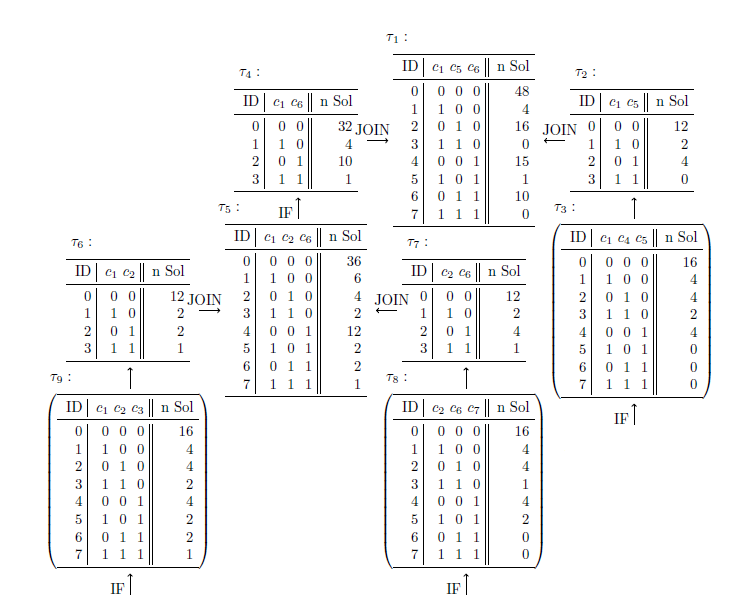
\includegraphics[width=0.6\linewidth]{images/DualDA43.png}
		\caption{Handcrafted \#SAT example-run from Markus Zisser\footnote{"Solving \#SAT on the GPU with Dynamic Programming and OpenCL",\\ Diploma Markus Zisser 2018 Technische Universit�t Wien, p.33}}
		\label{fig:dualda43}
	\end{figure}
	
\end{frame}
\begin{frame}
	\frametitle{Existing Visualization}
	\begin{figure}
		\centering
		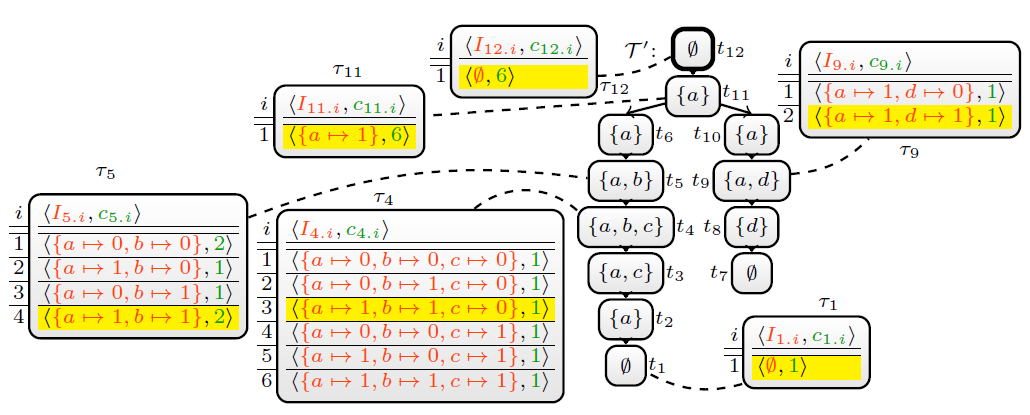
\includegraphics[width=\linewidth]{images/dpdbVisuSat.png}
		\caption{Handcrafted \#SAT example-run from dpdb\footnote{"Exploiting Database Management Systems and Treewidth for Counting",\\ Fichte, Hecher, Thier, Woltran} }
		\label{fig:dpdbVisuSat}
	\end{figure}
	
	
\end{frame}

%%%%%%%%%%%%%%%%%%%%%
\section{Background}
\begin{frame}
	\frametitle{Background}

\end{frame}

%%
\subsection{\#SAT and WMC}
\begin{frame}
	\frametitle{(Weighted) Model-Counting}
\end{frame}

\begin{frame}
	\frametitle{Graphs for Boolean Formulas}
	\smallskip
	\begin{itemize}
		\item {\color{blue} Example set of CNF-clauses:}\smallskip\\
		{\tiny $\{\text{c1}=\{\text{v1},\text{v3},\neg \text{v4}\},\text{c2}=\{\neg \text{v1},\text{v6}\},\text{c3}=\{\neg \text{v2},\neg \text{v3},\neg \text{v4}\},\text{c4}=\{\neg \text{v2},\text{v6}\},\text{c5}=\{\neg \text{v3},\neg \text{v4}\},\text{c6}=\{\neg \text{v3},\text{v5}\},\text{c7}=\{\neg \text{v5},\neg \text{v6}\},\text{c8}=\{\text{v5},\text{v7}\}\}
			$
		}
	\end{itemize}
	\begin{figure}
		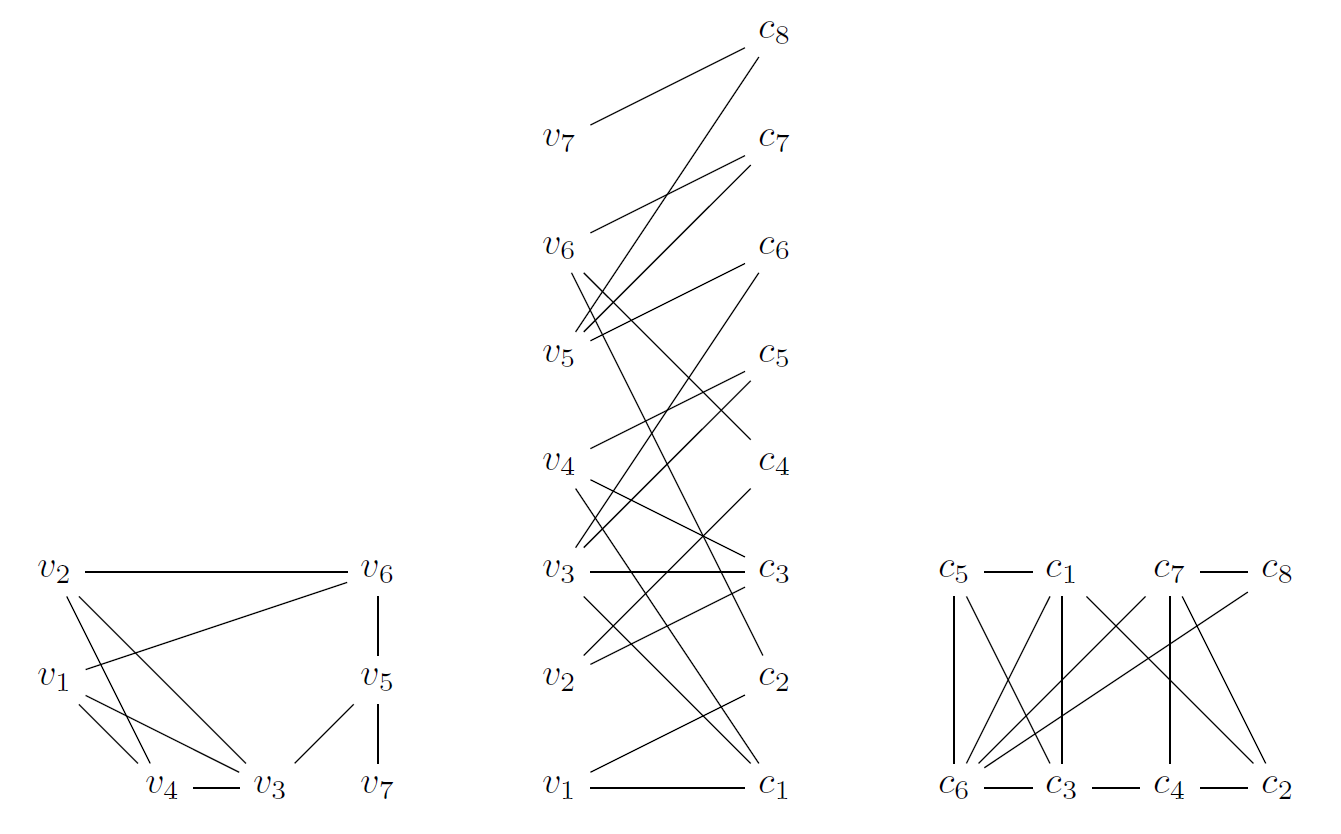
\includegraphics[height=0.5\textheight]{images/DAGraphs.png}
		\caption{The primal (left), incidence (middle) and dual (right) graph}
	\end{figure}
	%\footnotesize{Equivalent CNF}
	%{\tiny $(\neg \text{v1}\lor \neg \text{v3})\land (\neg \text{v1}\lor \text{v6})\land (\text{v1}\lor \neg \text{v4})\land (\neg \text{v2}\lor \neg \text{v5})\land (\neg \text{v2}\lor \text{v6})\land (\neg \text{v3}\lor \neg \text{v4})\land (\neg \text{v3}\lor \text{v5})\land (\neg \text{v5}\lor \neg \text{v6})\land (\text{v5}\lor \text{v7})$}
	
\end{frame}

%%
\subsection[TD]{Tree decomposition}
\begin{frame}
	\frametitle{Tree Decompositions}
	{\color{blue}\emph{Parameterized Complexity and its Applications in Practice} \\
		From Foundations to Implementations \\
		Johannes K. Fichte \\
		TU Dresden, Germany \\
		Jakarta, Indonesia \\
		{Summer 2019 (May 6th - May 16th)}
	}
	pages 162-174\\
	\bigskip
	\emph{Backup}: VC tree vs graph - example p69, 128
\end{frame}
%{
%	\setbeamercolor{background canvas}{bg=}
%	\includepdf[pages=162-174]{"images/Lecture_pcgp_Summer_2019.pdf"}
%}

\subsection{Example Vertex cover}
\begin{frame}
	\frametitle[Vertex Cover]{Example: Vertex-Cover problem}

\end{frame}
%%
\subsection[Courcelle]{Courcelle's theorem}
\begin{frame}
	\frametitle{Courcelle's theorem}

%	\begin{quotation}
%		Every graph property definable in monadic second-order logic (MSO) is decidable in linear time on graphs of bounded treewidth. \\
%		\hfill {\small Courcelle, Bruno (1990)}\footnote{Courcelle, Bruno "The monadic second-order logic of graphs. I. Recognizable sets of finite graphs",\\ Information and Computation, 85 (1990) no. 1: 12-75}
%	\end{quotation}

	\medskip
	For all $k \in \mathbb{N}$ and MSO-sentences F is the decision problem for a given graph G, whether $G \models F$ is true, in time $2^{p(tw(G))} \cdot |G|$ with a polynom p decidable.
	\medskip
	\begin{itemize}

		\item \emph{drawback:} still expensive ($2^{p(tw G)}$, $2^{2^{(\#Q)}}$, large constants) \smallskip 
		\item usage:

	\end{itemize}
	\begin{figure}
		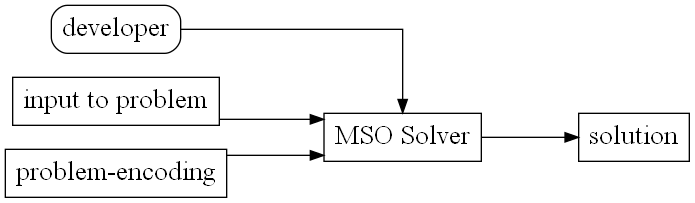
\includegraphics[height=0.2\textheight]{images/UsageCourcelle.gv.png}
		\caption{Implementation of the theorem}
	\end{figure}
\end{frame}


%%%%%%%%%%%%%%%%%%%%%%%
\section{Implementations}

\subsection{gpusat2}
\begin{frame}
	\frametitle{gpuSAT2 - Improving Upon Previous Ideas }
	%Architecture of our DP-based solver for parallel execution. Yellow colored
	%boxes indicate tasks that are required as initial step for the DP-run or to nally read the
	%model count from the computed results. The parts framed by a dashed box illustrate the
	%DP-part. Boxes colored in red indicate computations that run on the CPU. Boxes colored
	%in blue indicate computations that are executed on the GPU (with waiting CPU).
	\begin{figure}
		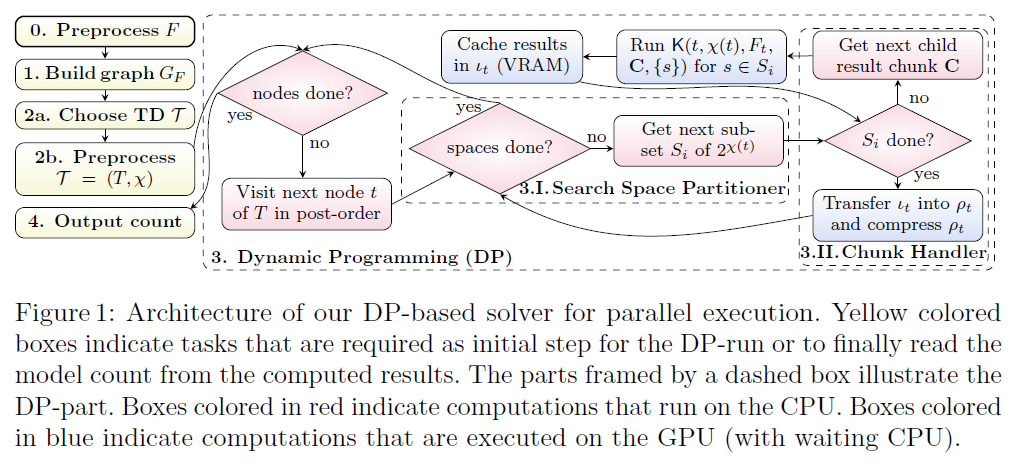
\includegraphics[height=0.3\textheight]{images/gpusat2DP.png}
	\end{figure}
	\begin{minipage}{0.49\textwidth}
		\begin{itemize}

			\item only primal graph { \small (simpler solving DP)}
			\item customized tree decompositions
			\item adapted memory-management
			\item improved precision handling

		\end{itemize}
	\end{minipage}
	\begin{minipage}{0.49\textwidth}
		%Runtime for the top 5 sequential and all parallel solvers over all the #Sat
		%instances with pmc preprocessor. The x-axis refers to the number of instances and the
		%y-axis depicts the runtime sorted in ascending order for each solver individually.
		\begin{figure}
			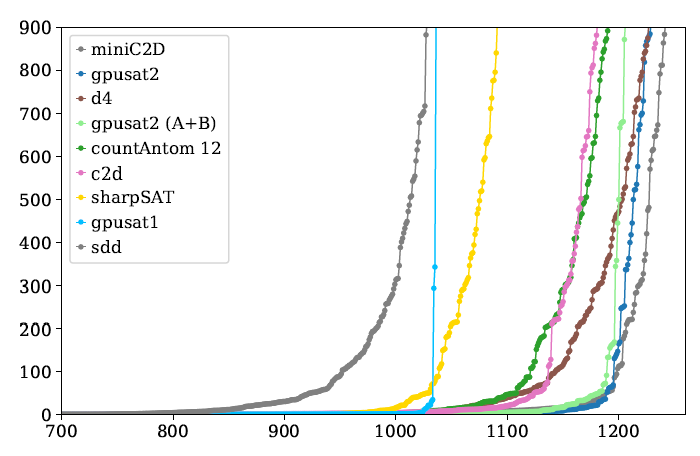
\includegraphics[width=\linewidth]{images/gpusat2Runtime.png}
		\end{figure}
	\end{minipage}

\end{frame}
%%
\subsection{dpdb}
\begin{frame}
	\frametitle{dpdb}
	{\color{blue}Using databases for intermediate results} \medskip\\
	%The idea of dpdb is to use database
	%management systems (DBMS) for table manipulation, which makes it (1) easy
	%and elegant to perform rapid prototyping for problems, and (2) allows to leverage
	%from decades of database theory and database system tuning. It turned out that
	%all the cases that occur in dynamic programming can be handled quite elegantly
	%with plain SQL queries. Our system dpdb can be used for both decision and
	%counting problems, thereby also considering optimization. We see our system
	%particularly well-suited for counting problems, especially, since it was shown
	%that for model counting (#Sat) instances of practical relevance typically have
	%small treewidth [23]. In consequence, we carried out preliminary experiments
	%on publicly available instances for
	\begin{minipage}{0.1\textwidth}
		\hfill
	\end{minipage}
	\begin{minipage}{0.35\textwidth}
		\begin{itemize}
			\item SAT
			\item \#SAT
			\item Vertex cover
		\end{itemize}
	\end{minipage}\hfill
	\begin{minipage}{0.54\textwidth}

		\begin{figure}
			\centering\hfill
			\begin{subfigure}[b]{\textwidth}
				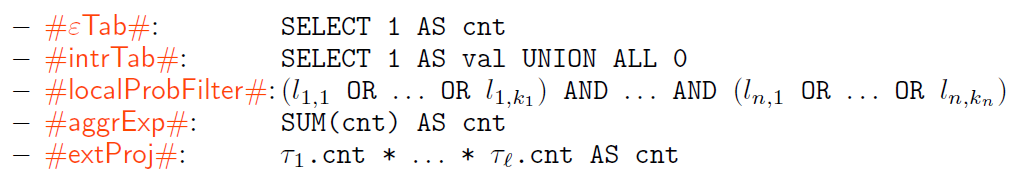
\includegraphics[width=\linewidth]{images/dpdbSSat.png}
				\caption{Problem \#SAT}

			\end{subfigure}\hfill\\
			\begin{subfigure}[b]{\textwidth}
				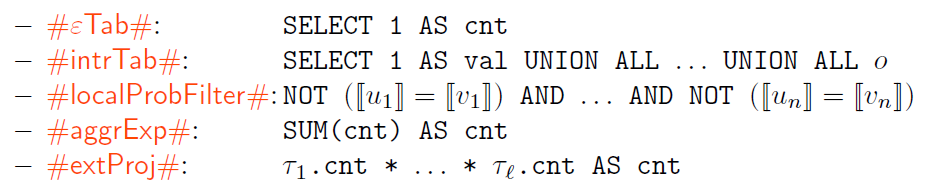
\includegraphics[width=0.8\linewidth]{images/dpdbOCol.png}
				\caption{Problem \#o-Col}

			\end{subfigure}\hfill\\
			\begin{subfigure}[b]{\textwidth}
				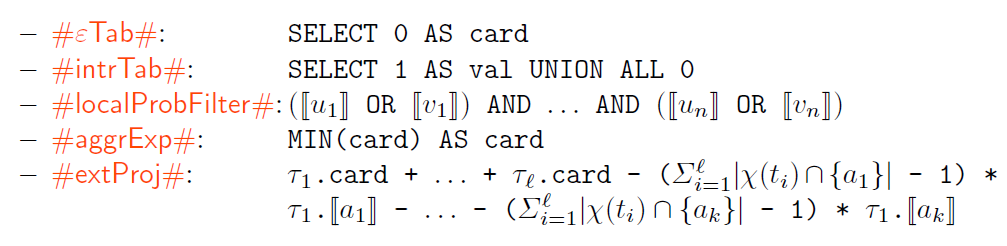
\includegraphics[width=0.8\linewidth]{images/dpdbMinVC.png}
				\caption{Problem MinVC}

			\end{subfigure}
		\end{figure}

	\end{minipage}
	\medskip \\
	github: \url{https://github.com/hmarkus/dp_on_dbs}
\end{frame}


%%%%%%%%%%%%%%%%%%%%%%%
\section{Challenge}
\begin{frame}
	\frametitle{Challenge1}
	\medskip
	
\end{frame}

\begin{frame}
	\frametitle{Challenge2}
	\medskip
	
\end{frame}

\begin{frame}
	\frametitle{Challenge3}
	\medskip
	
\end{frame}

%%%%%%%%%%%%%%%%%%%%%%%
\section{Outlook}
\begin{frame}
	\frametitle{Outlook}
	\medskip
	for relevant problems the static graph visualization will become to complicated.

\end{frame}
%%%%%%%%%%%%%%%%%%%%%%%

\begin{frame}
	\medskip
	\frametitle{Benchmark}
	{\color{blue}Performance of all three programs on \#SAT instances:} \medskip\\
	\begin{figure}
		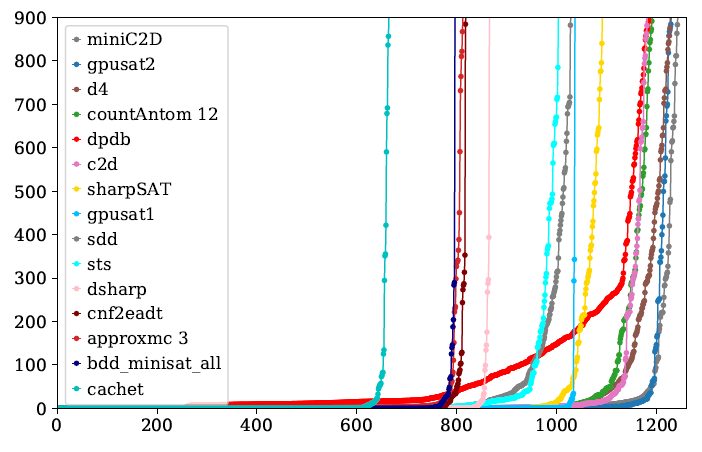
\includegraphics[width=0.8\linewidth]{images/dpdbRuntime.png}
	\end{figure}
\end{frame}

%%%%%%%%%%%%%%%%%%%%%%%
\section{BIBLIOGRAPHY}
\begin{frame}
	\frametitle{Bibliography}
	\medskip
	
\end{frame}



%%%%%%%%%%%%%%%%%%%%%%%%
\bgroup
\setbeamercolor{background canvas}{bg=black}
\begin{frame}[plain]{}
\end{frame}
\egroup

\end{document}